
\section{Σχεσιακό μοντέλο}

\subsection{Πεδία ορισμού}


\begin{tabular}{|p{6cm}|p{8cm}|}
\hline
  \textbf{Πεδίο Ορισμού} & \textbf{Τύπος}         \\ \hline
  Ακέραιος               & INT                    \\ \hline
  Όνομα                  & VARCHAR(40)            \\ \hline
  Δυαδικό                & ENUMERATED\{Ναι, Όχι\} \\ \hline
  Κείμενο                & VARCHAR(140)           \\ \hline
  Διεύθυνση              & VARCHAR(35)            \\ \hline
  Ώρα                    & TIME                   \\ \hline
  Ημερομηνία             & DATE                   \\ \hline
  Τηλεφωνο               & VARCHAR(14)            \\ \hline
  Τιμή                   & DEC(2,2)               \\ \hline
  email                  & VARCHAR(30)            \\ \hline
  pass                   & VARCHAR(15)            \\ \hline
  Αριθμός16              & DEC(16,0)              \\ \hline
  Αριθμός3               & DEC(3,0)               \\ \hline
  Εισιτήρια              & VARCHAR(10)            \\ \hline
\end{tabular}

\subsection{Σχέσεις}

Παρακάτω παρουσιάζονται οι σχέσεις της EventsDB, όπως μεταφέρονται από
το μοντέλο οντοτήτων/ συσχετίσεων στην τρίτη κανονική τους μορφή.

\subsubsection*{Εκδήλωση}

\begin{tabular}{|p{6cm}|p{8cm}|}
  \multicolumn{2}{l}{\textbf{Γνωρίσματα:}}                          \\ \hline
  Όνομα                   & Τύπος                                   \\ \hline
  Κωδικός\_εκδήλωσης      & Ακέραιος                                \\ \hline
  Όνομα\_εκδήλωσης        & Όνομα                                   \\ \hline
  Ύπαρξη\_εισιτηρίου      & Διαδικό                                 \\ \hline
  Κοινό\_που\_απευθύνεται & Όνομα                                   \\ \hline
  Περιγραφή               & Κείμενο                                 \\ \hline
  Ημερομηνία              & Ημερομηνία                              \\ \hline
  Ώρα\_έναρξης            & Ώρα                                     \\ \hline
  Κωδικός\_τοπεθεσίας     & Ακέραιος                                \\ \hline
  Κωδικός\_ερμηνευτή      & Ακέραιος                                \\ \hline
  Κωδικός\_διοργανωτή     & Ακέραιος                                \\ \hline
  \multicolumn{2}{l}{\textbf{Περιορισμοί Ακεραιότητας:}}            \\ \hline
  Πρωτεύον Κλειδί         & Κωδικός\_εκδήλωσης                      \\ \hline
  Ξένα Κλειδιά            & Κωδικός\_τοποθεσίας -> Τοποθεσία        \\ \cline{2-2}
                          & Κωδικός\_Ερμηνευτή -> Καλλιτέχνης-Ομάδα \\ \cline{2-2}
                          & Κωδικός\_διοργανώτή -> Διοργανωτής      \\ \hline
\end{tabular}

\subsubsection*{Μουσική\_εκδήλωση}

\begin{tabular}{|p{6cm}|p{8cm}|}
  \multicolumn{2}{l}{\textbf{Γνωρίσματα:}}                   \\ \hline
  Όνομα                     & Τύπος                          \\ \hline
  Κωδικός\_εκδήλωσης        & Ακέραιος                       \\ \hline
  Ύπαρξη\_θέσεων\_καθημένων & Δυαδικό                        \\ \hline
  Είδος                     & Κείμενο                        \\ \hline
  Opening\_act              & Κείμενο                        \\ \hline
  \multicolumn{2}{l}{\textbf{Περιορισμοί Ακεραιότητας:}}     \\ \hline
  Πρωτεύον Κλειδί           & Κωδικός\_εκδήλωσης             \\ \hline
  Ξένα Κλειδιά              & Κωδικός\_εκδήλωσης -> Εκδήλωση \\ \hline
\end{tabular}

\subsubsection*{Θέατρο}

\begin{tabular}{|p{6cm}|p{8cm}|}
  \multicolumn{2}{l}{\textbf{Γνωρίσματα:}}               \\ \hline
  Όνομα               & Τύπος                            \\ \hline
  Κωδικός\_εκδήλωσης  & Ακέραιος                         \\ \hline
  Ύπαρξη\_θέσεων\_VIP & Δυαδικό                          \\ \hline
  Διάρκεια            & Ακέραιος                         \\ \hline
  \multicolumn{2}{l}{\textbf{Περιορισμοί Ακεραιότητας:}} \\ \hline
  Πρωτεύον Κλειδί     & Κωδικός\_εκδήλωσης               \\ \hline
  Ξένα Κλειδιά        & Κωδικός\_εκδήλωσης -> Εκδήλωση   \\ \hline
\end{tabular}

\subsubsection*{Αθλητική\_εκδήλωση}

\begin{tabular}{|p{6cm}|p{8cm}|}
  \multicolumn{2}{l}{\textbf{Γνωρίσματα:}}               \\ \hline
  Όνομα               & Τύπος                            \\ \hline
  Κωδικός\_εκδήλωσης  & Ακέραιος                         \\ \hline
  Ύπαρξη\_θέσεων\_VIP & Δυαδικό                          \\ \hline
  Άθλημα              & Κείμενο                          \\ \hline
  \multicolumn{2}{l}{\textbf{Περιορισμοί Ακεραιότητας:}} \\ \hline
  Πρωτεύον Κλειδί     & Κωδικός\_εκδήλωσης               \\ \hline
  Ξένα Κλειδιά        & Κωδικός\_εκδήλωσης -> Εκδήλωση   \\ \hline
\end{tabular}

\subsubsection*{Εισιτήριο}

\begin{tabular}{|p{6cm}|p{8cm}|}
  \multicolumn{2}{l}{\textbf{Γνωρίσματα:}}                     \\ \hline
  Όνομα              & Τύπος                                   \\ \hline
  Κωδικός\_εκδήλωσης & Ακέραιος                                \\ \hline
  Τύπος\_εισιτηρίου  & Εισιτήρια                               \\ \hline
  Τιμή               & Τιμή                                    \\ \hline
  \multicolumn{2}{l}{\textbf{Περιορισμοί Ακεραιότητας:}}       \\ \hline
  Πρωτεύον Κλειδί    & Κωδικός\_εκδήλωσης \& Τύπος\_εισιτηρίου \\ \hline
  Ξένο Κλειδί        & Κωδικός\_εκδήλωσης -> Εκδήλωση          \\ \hline
\end{tabular}


\subsubsection*{Τοποθεσία}

\begin{tabular}{|p{6cm}|p{8cm}|}
  \multicolumn{2}{l}{\textbf{Γνωρίσματα:}}               \\ \hline
  Όνομα                  & Τύπος                         \\ \hline
  Κωδικός\_τοποθεσίας    & Ακέραιος                      \\ \hline
  Όνομα\_τοποθεσίας      & Όνομα                         \\ \hline
  Εσωτερικός\_χώρος      & Δυαδικό                       \\ \hline
  Τηλέφωνο               & Τηλέφωνο                      \\ \hline
  Διεύθυνση              & Διεύθυνση                     \\ \hline
  Ύπαρξη\_υποδομών\_ΑΜΕΑ & Δυαδικό                       \\ \hline
  Τιμή\_μπύρας           & Τιμή                          \\ \hline
  Τιμή\_κρασιού          & Τιμή                          \\ \hline
  Τιμή\_Ποτού            & Τιμή                          \\ \hline
  \multicolumn{2}{l}{\textbf{Περιορισμοί Ακεραιότητας:}} \\ \hline
  Πρωτεύον Κλειδί        & Κωδικός\_τοποθεσίας           \\ \hline
\end{tabular}


\subsubsection*{Καλλιτέχνης-Ομάδα}

\begin{tabular}{|p{6cm}|p{8cm}|}
  \multicolumn{2}{l}{\textbf{Γνωρίσματα:}}               \\ \hline
  Όνομα              & Τύπος                             \\ \hline
  Κωδικός\_ερμηνευτή & Ακέραιος                          \\ \hline
  Ονοματεπώνυμο      & Όνομα                             \\ \hline
  Καταγωγή           & Όνομα                             \\ \hline
  \multicolumn{2}{l}{\textbf{Περιορισμοί Ακεραιότητας:}} \\ \hline
  Πρωτεύον Κλειδί    & Κωδικός\_ερμηνευτή                \\ \hline
\end{tabular}

\subsubsection*{Καλλιτέχνης}

\begin{tabular}{|p{6cm}|p{8cm}|}
  \multicolumn{2}{l}{\textbf{Γνωρίσματα:}}                       \\ \hline
  Όνομα                & Τύπος                                   \\ \hline
  Κωδικός\_ερμηνευτή   & Ακέραιος                                \\ \hline
  Είδος                & Όνομα                                   \\ \hline
  Ημερομηνία\_γέννησης & Ημερομηνία                              \\ \hline
  \multicolumn{2}{l}{\textbf{Περιορισμοί Ακεραιότητας:}}         \\ \hline
  Πρωτεύον Κλειδί      & Κωδικός\_ερμηνευτή                      \\ \hline
  Ξένο Κλειδί          & Κωδικός\_ερμηνευτή -> Καλλιτέχνης-Ομάδα \\ \hline
\end{tabular}

\subsubsection*{Ομάδα}

\begin{tabular}{|p{6cm}|p{8cm}|}
  \multicolumn{2}{l}{\textbf{Γνωρίσματα:}}                     \\ \hline
  Όνομα              & Τύπος                                   \\ \hline
  Κωδικός\_ερμηνευτή & Ακέραιος                                \\ \hline
  Όνομα\_υπευθύνου   & Όνομα                                   \\ \hline
  \multicolumn{2}{l}{\textbf{Περιορισμοί Ακεραιότητας:}}       \\ \hline
  Πρωτεύον Κλειδί    & Κωδικός\_ερμηνευτή                      \\ \hline
  Ξένο Κλειδί        & Κωδικός\_ερμηνευτή -> Καλλιτέχνης-Ομάδα \\ \hline
\end{tabular}


\subsubsection*{Φυσικό\_σημείο\_προπώλησης}

\begin{tabular}{|p{6cm}|p{8cm}|}
  \multicolumn{2}{l}{\textbf{Γνωρίσματα:}}               \\ \hline
  Όνομα            & Τύπος                               \\ \hline
  Κωδικός\_σημείου & Ακέραιος                            \\ \hline
  Όνομα\_σημείου   & Όνομα                               \\ \hline
  Τηλέφωνο         & Τηλέφωνο                            \\ \hline
  Διεύθυνση        & Διεύθυνση                           \\ \hline
  \multicolumn{2}{l}{\textbf{Περιορισμοί Ακεραιότητας:}} \\ \hline
  Πρωτεύον Κλειδί  & Κωδικός\_σημείου                    \\ \hline
\end{tabular}

\subsubsection*{Προπώληση}

\begin{tabular}{|p{6cm}|p{8cm}|}
  \multicolumn{2}{l}{\textbf{Γνωρίσματα:}}                    \\ \hline
  Όνομα              & Τύπος                                  \\ \hline
  Κωδικός\_σημείου   & Ακέραιος                               \\ \hline
  Κωδικός\_εκδήλωσης & Ακέραιος                               \\ \hline
  Πρωτεύον Κλειδί    & Κωδικός\_σημείου \& Κωδικός\_εκδήλωσης \\ \hline
  Ξένο Κλειδί        & Κωδικός\_σημείου -> Φυσικό\_σημείο\_προπώλησης
                                                              \\ \hline
                     & Κωδικός\_εκδήλωσης -> Εκδήλωση         \\ \hline
\end{tabular}


\subsubsection*{Διοργανωτής}

\begin{tabular}{|p{6cm}|p{8cm}|}
  \multicolumn{2}{l}{\textbf{Γνωρίσματα:}}               \\ \hline
  Όνομα               & Τύπος                            \\ \hline
  Κωδικός\_διοργανωτή & Ακέραιος                         \\ \hline
  Όνομα\_εταιρίας     & Όνομα                            \\ \hline
  email               & email                            \\ \hline
  Τηλέφωνο            & Τηλέφωνο                         \\ \hline
  password            & pass                             \\ \hline
  \multicolumn{2}{l}{\textbf{Περιορισμοί Ακεραιότητας:}} \\ \hline
  Πρωτεύον Κλειδί     & Κωδικός\_διοργανωτή              \\ \hline
\end{tabular}


\subsubsection*{Χρήστης}

\begin{tabular}{|p{6cm}|p{8cm}|}
  \multicolumn{2}{l}{\textbf{Γνωρίσματα:}}               \\ \hline
  Όνομα           & Τύπος                                \\ \hline
  Κωδικός\_χρήστη & Ακέραιος                             \\ \hline
  Ονοματεπώνυμο   & Όνομα                                \\ \hline
  email           & email                                \\ \hline
  password        & pass                                 \\ \hline
  \multicolumn{2}{l}{\textbf{Περιορισμοί Ακεραιότητας:}} \\ \hline
  Πρωτεύον Κλειδί & Κωδικός\_χρήστη                      \\ \hline
\end{tabular}


\subsubsection*{Κάρτα}

\begin{tabular}{|p{6cm}|p{8cm}|}
  \multicolumn{2}{l}{\textbf{Γνωρίσματα:}}               \\ \hline
  Όνομα              & Τύπος                             \\ \hline
  Αριθμός\_κάρτας    & Αριθμός16                         \\ \hline
  Αριθμός\_ασφαλείας & Αριθμός3                          \\ \hline
  Διεύθυνση          & Διεύθυνση                         \\ \hline
  Κωδικός\_χρήστη    & Ακέραιος                          \\ \hline
  \multicolumn{2}{l}{\textbf{Περιορισμοί Ακεραιότητας:}} \\ \hline
  Πρωτεύον Κλειδί    & Αριθμός\_κάρτας                   \\ \hline
  Ξένα Κλειδιά       & Κωδικός\_χρήστη -> Χρήστης        \\ \hline
\end{tabular}

\subsubsection*{Αγορά}

\begin{tabular}{|p{6cm}|p{8cm}|}
  \multicolumn{2}{l}{\textbf{Γνωρίσματα:}}                   \\ \hline
  Όνομα              & Τύπος                                 \\ \hline
  Κωδικός\_εκδήλωσης & Ακέραιος                              \\ \hline
  Κωδικός\_χρήστη    & Ακέραιος                              \\ \hline
  Τύπος\_εισιτηρίου  & Εισιτήρια                             \\ \hline
  \multicolumn{2}{l}{\textbf{Περιορισμοί Ακεραιότητας:}}     \\ \hline
  Πρωτεύον Κλειδί    & Κωδικός\_χρήστη \& Κωδικός\_εκδήλωσης \\ \hline
  Ξένα Κλειδιά       & Κωδικός\_χρήστη -> Χρήστης            \\ \hline
                     & Κωδικός\_εκδήλωσης -> Εισιτήριο       \\ \hline
                     & Τύπος\_εισιτηρίου -> Εισιτήριο        \\ \hline
\end{tabular}

\subsubsection*{Ενδιαφέρον}

\begin{tabular}{|p{6cm}|p{8cm}|}
  \multicolumn{2}{l}{\textbf{Γνωρίσματα:}}                   \\ \hline
  Όνομα              & Τύπος                                 \\ \hline
  Κωδικός\_εκδήλωσης & Ακέραιος                              \\ \hline
  Κωδικός\_χρήστη    & Ακέραιος                              \\ \hline
  \multicolumn{2}{l}{\textbf{Περιορισμοί Ακεραιότητας:}}     \\ \hline
  Πρωτεύον Κλειδί    & Κωδικός\_χρήστη \& Κωδικός\_εκδήλωσης \\ \hline
  Ξένα Κλειδιά       & Κωδικός\_χρήστη -> Χρήστης            \\ \hline
                     & Κωδικός\_εκδήλωσης -> εκδήλωση        \\ \hline
\end{tabular}

\subsection{Σχεσιακό Σχήμα}

\begin{figure}[H]
  \centering
  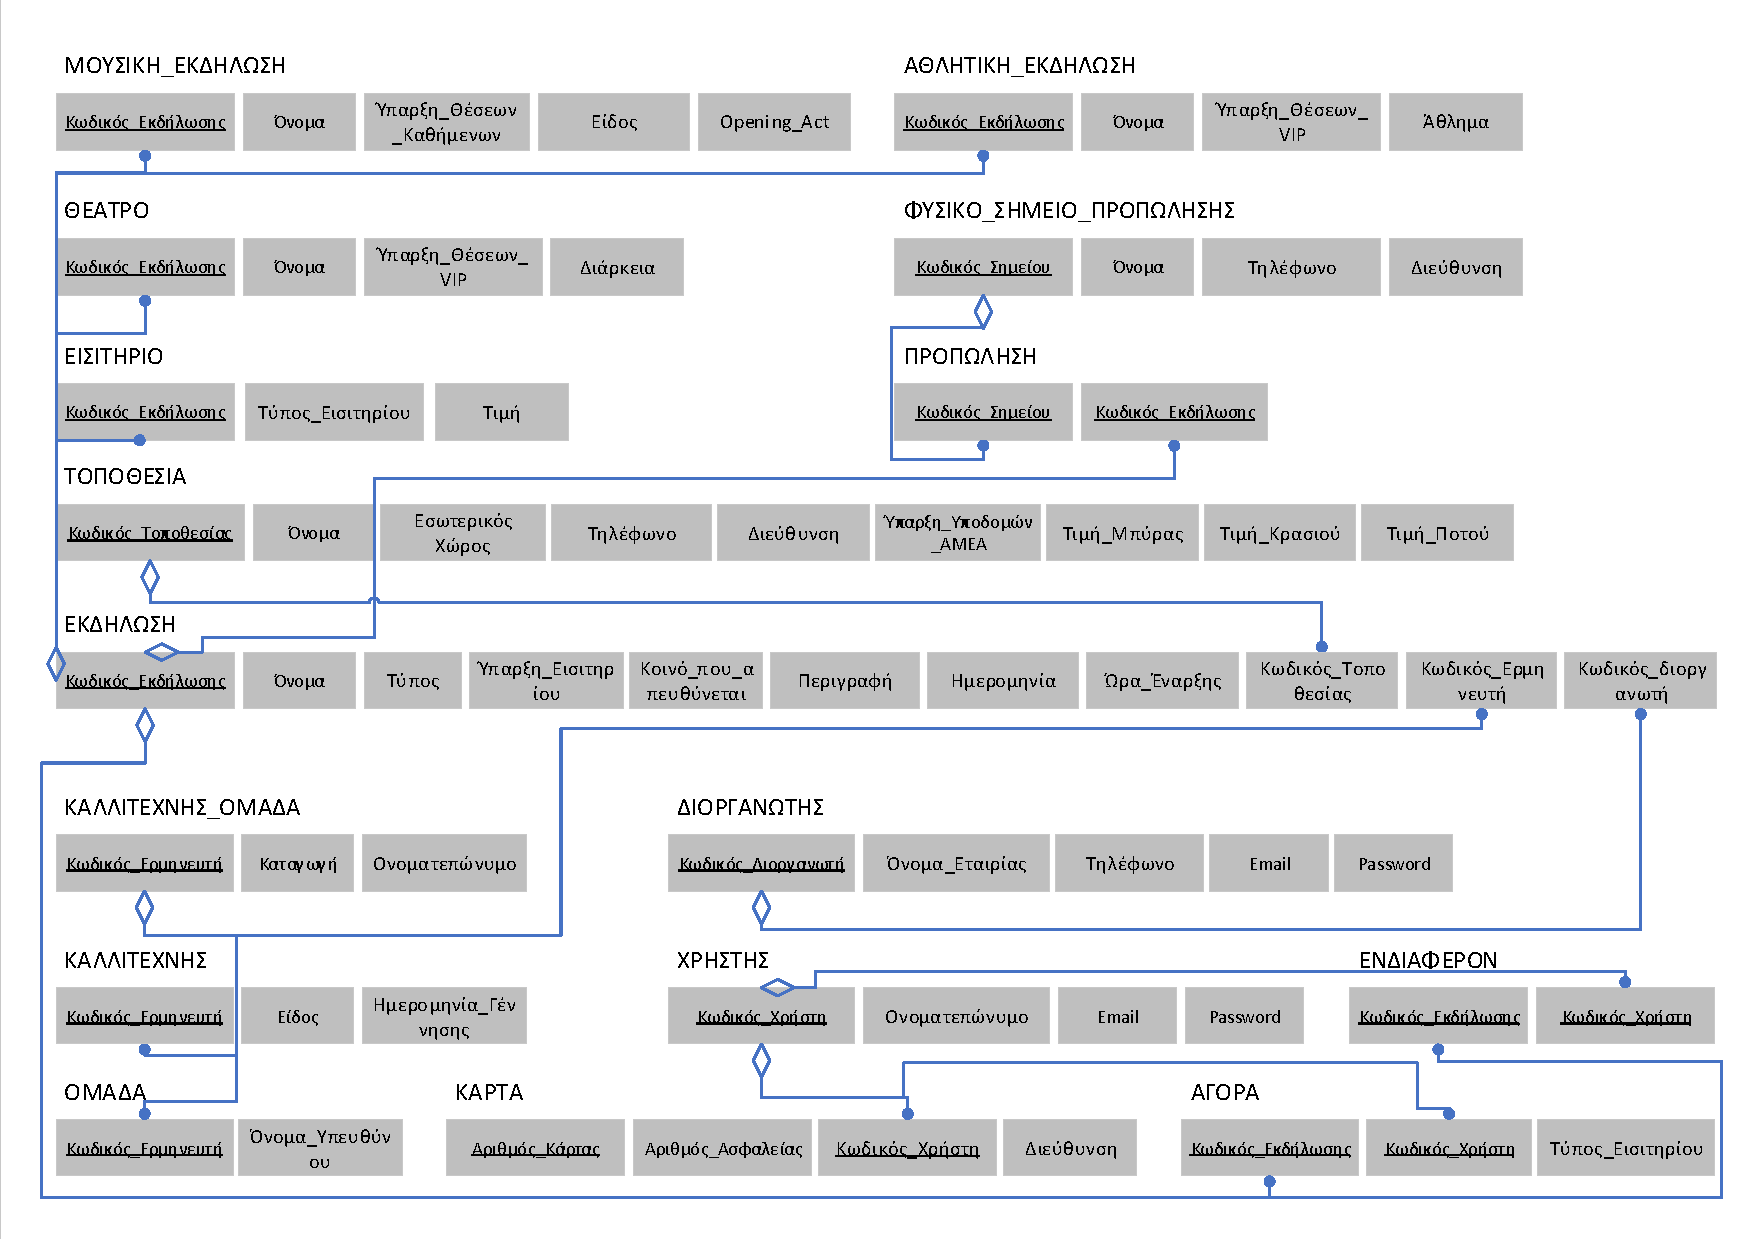
\includegraphics[width=\linewidth]{Relations.pdf}
  \caption{Σχεσιακό μοντέλο}
\end{figure}

\subsection{Όψεις}

Παρακάτω παρουσιάζονται κάποιες ενδεικτικές όψεις της βάσης δεδομένων
οι οποίες δίνουν μια πολύ καλή εικόνα για το πως όλες οι σχέσεις
συνδέονται μεταξύ τους.

Η βασικότερη όψη είναι αυτή όπου προβάλει όλες τις πληροφορίες μιας
εκδήλωσης από όλες τις σχέσεις. Λόγω των διαφορετικών υποτύπων μιας
εκδήλωσης, για λόγους καθαρότητας, δημιουργούνται τέσσερις όψεις, μία
για κάθε υποτύπο.

\begin{equation}
  \begin{split}
    &\text{EVENT} \leftarrow \sigma_{<\text{Τύπος} =
      \text{"Εκδήλωση"}>}\text{Εκδήλωση} \\
    &\text{ή}\\
    &\text{EVENT} \leftarrow \sigma_{<\text{Τύπος} = \text{"Θεατρική
        Εκδήλωση"}>}\text{Εκδήλωση} \bowtie \text{Θέατρο} \\
    &\text{ή} \\
    &\text{EVENT} \leftarrow \sigma_{<\text{Τύπος} = \text{"Αθλητική
        Εκδήλωση"}>}\text{Εκδήλωση} \bowtie \text{Αθλητική\_εκδήλωση} \\
    &\text{ή} \\
    &\text{EVENT} \leftarrow \sigma_{<\text{Τύπος} = \text{"Μουσική
        Εκδήλωση"}>}\text{Εκδήλωση} \bowtie \text{Μουσική\_εκδήλωση} \\
    &\text{και} \\
    &\text{EVENT} \bowtie \text{Τοποθεσία} \bowtie
    \text{Καλλιτέχνης-Ομάδα} \bowtie \text{Διοργ} \\
  \end{split}
\end{equation}

Όπου Διοργ είναι μια όψη της σχέσης Διοργανοτής όπου εμφανίζει μόνο
τις αρμόζουσες πληροφορίες των διοργανωτών στους υπόλοιπους χρήστες.

\begin{equation}
  \text{Διοργ} \leftarrow \Pi_{<\text{Κωδικός\_διοργανωτή,
      Όνομα\_εταιρίας, email, Τηλέφωνο}>}\text{Διοργανωτής}
\end{equation}


% Παρακάτω παρουσιάζονται κάποιες ενδεικτικές όψεις της βάσης δεδομένων
% οι οποίες δίνουν μια πολύ καλή εικόνα για το πως όλες οι σχέσεις
% συνδέονται μεταξύ τους. Αρκετές όψεις έχουν πολλές ομοιότητες μεταξύ
% τους και γι' αυτόν τον λόγο θα παρουσιαστούν ενδεικτικά κάποιες από
% αυτές.

% \begin{itemize}

% \item Μία βασική όψη που θα διατίθεται μόνο σε διοργανωτές είναι η
%   προβολή όλων των Καλλιτεχνών-Ομάδων που σχετίζονται με εκδηλώσεις
%   που διοργανώνουν.
  
%   \begin{equation} \label{eq1}
%     \begin{split}

%       &\Pi_{<\text{Όνομα\_εκδήλωσης, Ημερομηνία, Ώρα έναρξης, Ονοματεπώνυμο,
%           Καταγωγή, }>}A
%       &A \leftarrow \text{Εκδήλωση} \bowtie
%       \text{Καλλιτέχνης-Ομάδα} \bowtie
%       \sigma_{<\text{Όνομα\_τοποθεσίας} = \text{"Τα Ξύδια"}>}
%       \text{Τοποθεσία}
%       \\
      
%     \end{split}
%   \end{equation}

% (ΚΑΛΛΙΤΕΧΝΗΣ-ΟΜΑΔΑ: Ονοματεπώνυμο, Καταγωγή + ΕΚΔΗΛΩΣΗ: Όνομα, Ημερομηνία,
% Ώρα\_Έναρξης \+ ΟΜΑΔΑ: Όνομα\_Υπευθύνου)

% \item Μια άλλη γενική όψη, προσβάσιμη τόσο από διοργανωτές, όσο και
%   από χρήστες (εγγεγραμμένους και μη) είναι η προβολή των βασικών
%   στοιχείων όλων των εκδηλώσεων σε συνδυασμό με τις πληροφορίες
%   τοποθεσίας τους.

% \(ΕΚΔΗΛΩΣΗ: Όνομα, Τύπος, Κοινό\_που\_απευθύνεται,
% Ημερομηνία, Ώρα\_Έναρξης \+ ΤΟΠΟΘΕΣΙΑ: Όνομα, Εσωτερικός\_Χώρος, Τηλέφωνο,
% ΔΙεύθυνση)

% \item Οι εγγεγραμμένοι χρήστες θα μπορούν να προβάλλουν μια λίστα με
%   τις εκδηλώσεις για τις οποίες έχουν αγοράσει εισιτήριο.
  
% (ΚΑΡΤΑ: Αριθμός\_Κάρτας \+ ΕΚΔΗΛΩΣΗ: Όνομα, Τύπος, Ημερομηνία, Ώρα\_Έναρξης
% \+ ΕΙΣΙΤΗΡΙΟ: Τύπος\_Εισιτηρίου, Τιμή)

% \item Οι εγγεγραμμένοι χρήστες επίσης θα έχουν τη δυνατότητα να
%   προβάλλουν τις εκδηλώσεις για τις οποίες έχουν δείξει ενδιαφέρον.
  
% (ΕΚΔΗΛΩΣΗ: Όνομα, Τύπος, Ύπαρξη\_Εισιτηρίου, Ημερομηνία, Ώρα\_Έναρξης
% \+ ΤΟΠΟΘΕΣΙΑ: Όνομα, Τηλέφωνο, Διεύθυνση \+ ΦΥΣΙΚΟ\_ΣΗΜΕΙΟ\_ΠΡΟΠΩΛΗΣΗΣ:
% Όνομα, Τηλέφωνο, Διεύθυνση \+ ΕΙΣΙΤΗΡΙΟ: Τύπος\_Εισιτηρίου, Τιμή)

% \end{itemize}


%%% Local Variables:
%%% mode: latex
%%% TeX-master: "main"
%%% TeX-engine: xetex
%%% End:
